\chapter{Domain}
\label{chap:domain}

This chapter begins with a high level description of the domain. This is followed by a description of the schema in the relational database of CIMS and a depiction of the data influx rate in CIMS. The chapter ends with potential uses cases for an archive solution and the database queries needed for those use cases.
\begin{figure}[h!]
\centering
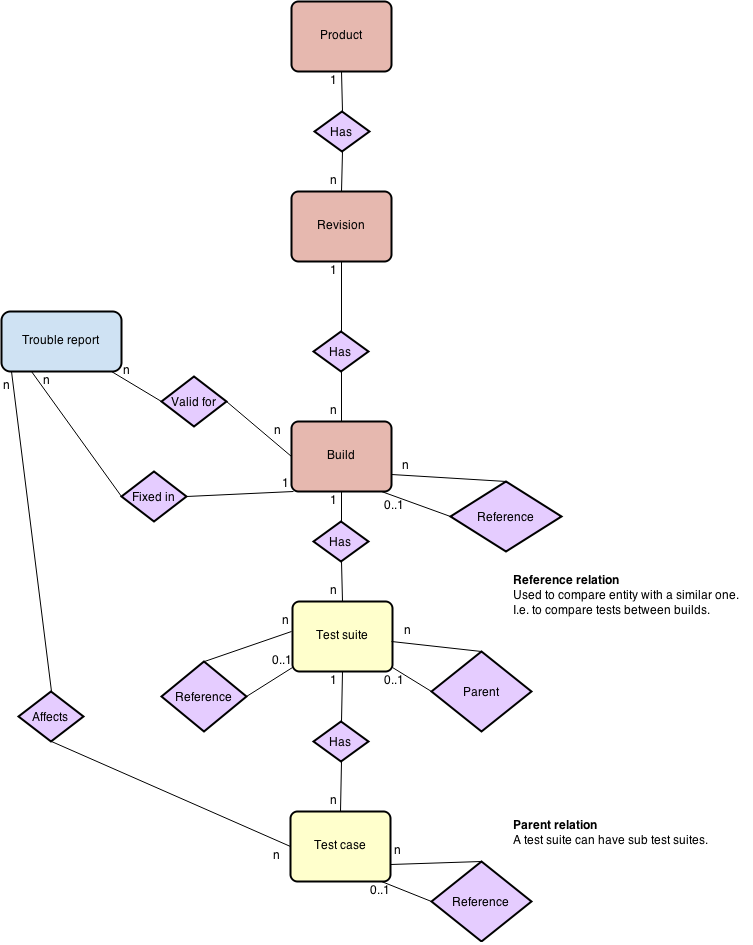
\includegraphics[scale=0.45]{figure/er_diagram.png}
\caption{High level diagram of the domain.}
\label{fig:er}
\end{figure}

\section{High level schema}
For the feasibility of this study, the domain of CIMS has been narrowed to some key entities, which are the following; products, revisions, builds, test suites, test cases and trouble reports. Excluding trouble reports, these entities form a hierarchical structure as seen in figure~\ref{fig:er}. Products are at the top of this hierarchy. They represent the different software systems that are being developed at Ericsson. Products are developed iteratively, where a released iteration is called a revision. At the revision level, developers makes changes to source code, configuration, tests etc.\ which are then checked into a revision control system and subsequently built and tested. This is referred to in domain terms as a build. Each build runs a number of test suites, which in turn consist of a number of test cases.

As has been noted, a trouble report sits outside of the hierarchy. This entity represents a bug or defect which arrives from external (i.e.\ a customer) or internal sources. It can be mapped to different entities from products down to specific test cases. Trouble reports are handled by implementing a fix in a specific build.

\section{Existing relational implementation}
The relational database schema in use by CIMS represents the above mentioned entities in a different abstraction. Representation of these entities is described in depth in the sections below. 
The schema of the relational database in CIMS is presented in figure~\ref{fig:sql}.

\hiddensubsection{Job}
A job in the relational implementation does not have a directly corresponding entity in the high level diagram visualized in figure~\ref{fig:er}. The job is a technical entity that groups related test cases and test suites. As seen in figure~\ref{fig:job} a job is represented by the job table which is linked to a build via the build\_job\_mapping table. 

\begin{figure}[h!]
\centering
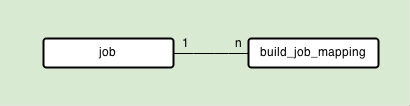
\includegraphics[scale=0.5]{figure/job.jpg}
\caption{Diagram of tables related to jobs.}
\label{fig:job}
\end{figure}

\hiddensubsection{Build}
In the relational database, a build is represented by the build table. Each build can possess a number of artifacts and deliverable events, as seen in figure~\ref{fig:build}. An artifact can for instance be the path to a binary file that is included in the build. The deliverable\_event table is for defining which deliverables (i.e.\ trouble reports) that belongs to the build.
\begin{figure}[h!]
\centering
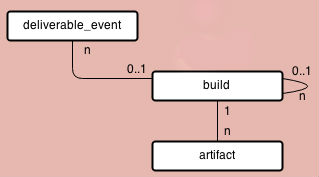
\includegraphics[scale=0.5]{figure/build.jpg}
\caption{Diagram of tables related to builds.}
\label{fig:build}
\end{figure}

\hiddensubsection{Deliverable}
A deliverable in the relational database represents a trouble report described in figure~\ref{fig:er}. As seen in figure~\ref{fig:deliverable} a deliverable is defined by the following tables; deliverable, deliverable\_event, deliverable\_status and deliverable\_affected\_testcase. These tables contain normalized data about a deliverable. 
\begin{figure}[h!]
\centering
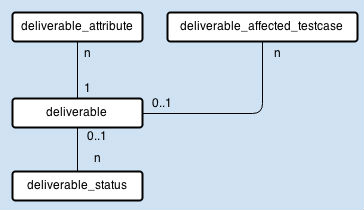
\includegraphics[scale=0.5]{figure/deliverable.jpg}
\caption{Diagram of tables related to trouble reports.}
\label{fig:deliverable}
\end{figure}

\hiddensubsection{Job event}
The relational representation of a test case and test suite described in figure~\ref{fig:er} is the job event entity. Each test case and test suite registered in CIMS becomes a job event and the job events that are related forms a tree structure describing the execution of a test suite. As seen in figure~\ref{fig:job_event} a job event is represented by the job\_event table which is linked to multiple tables containing normalized data about the job event.
\label{sec:jobEvent}
\begin{figure}[h!]
\centering
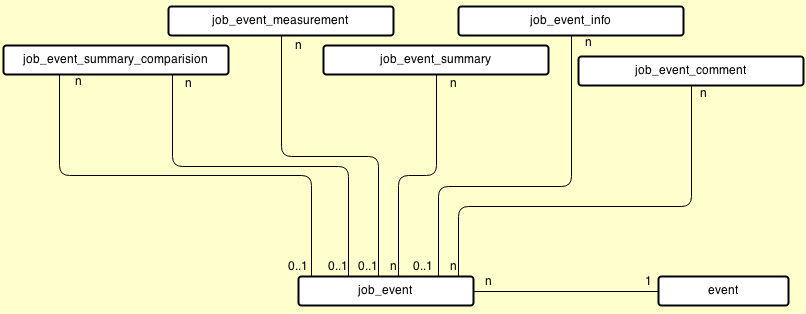
\includegraphics[scale=0.5]{figure/job_event.jpg}
\caption{Diagram of tables related to test cases.}
\label{fig:job_event}
\end{figure}







\section{Use cases}
\label{sec:usecases}
A number of use cases have been identified for the archive that can provide business value to Ericsson and thereby motivates why saving data in an archive is viable. These include the ability to have information about each build, even builds that were executed years ago and the ability to perform analysis on larger data sets. 

The first use case is an important part in Ericsson's process of managing bugs that is found by the customer running live versions of a product. Even if CI leads to shorter release cycles, the lead time of deploying new software at a customer is still relatively long. It can also be the case that the customer doesn't have the need or resources to upgrade to a newer software version. This leads to that customers can use software that was released years ago. When a customer finds a bug or their system crashes, in order to quickly fix that bug, it is crucial to have all information about that particular build in use by the customer. Information such as the outcome of all tests performed, warnings in the build procedure are examples of such necessary information. 

The second use case can give Ericsson further insight in the quality and trends in their development processes. For Ericsson to be able to improve in their processes of building and designing software, meta data of the software's developed needs to be analyzed. The data in CIMS needs to be correlated with other sources of information, such as the trouble report system. This use case will provide value to roles such as managers, they can in nearly real time see if the quality of the produced software is declining or increasing compared to earlier measurements and can be more certain that it is not just a temporary event because they will have the ability of doing analysis on years of data. 


\hiddensubsection{Queries}
In order to manage the use cases mentioned in the section above, the archive needs to support a large set of queries. Below we describe one of the more interesting queries, namely looking up a test case history. It is described in domain terms and in terms of the relational implementation of CIMS. More queries can be seen in appendix A.


\hiddensubsubsection{Get test case history}
\label{q:tchistory}
This query should return the history of a test case, identified by its name. It should group the results by product and for each of these it should show the builds containing the specific test case and the verdict of the test case in that build. This query cannot be expressed as a single SQL statement and is implemented on the application level in CIMS by performing several SQL queries and building a dictionary with the results. Pseudo code for this query is show in figure~\ref{code:tc_history}

\begin{figure}[ht]
\begin{mdframed}
\begin{verbatim}
job_events = 
    SELECT * FROM cims_job_event 
    WHERE name = 'my_test_case'

// List comprehension
job_names = job_event.job_name FOR job_event IN job_events 

jobs = SELECT * FROM cims_job WHERE job_name IN job_names

// List comprehension
root_job_event_ids = job.root_jobevent_id FOR job IN jobs

root_job_events = 
    SELECT * FROM job_event WHERE id IN root_job_event_ids

builds = 
    SELECT cims_build.* FROM cims_build
    INNER JOIN cims_build_job_mapping
    ON cims_build_job_mapping.build_id = cims_build.id
    WHERE cims_build_job_mapping.job_name IN job_names

(Use list of job_events, jobs, 
root job events and builds to create result dictionary)
\end{verbatim}
\end{mdframed}
\caption{Pseudo code describing the test case history query.}
\label{code:tc_history}
\end{figure}

\section{Data generation rate}
\label{datagenrate}
We end this chapter by presenting the current data generation rates for builds and events (i.e.\ test cases and trouble reports). This is useful so as to put the growth trends in a context. One part in designing a solution is to be aware of these trends. In the introduction the accumulated amount of job events where shown in figure~\ref{fig:jeTrend}. The figure was chosen to illustrate the overall current data growth trend for one specific product at Ericsson. The cause for this trend is twofold. First of all the amount of builds registered every month is increasing, as can be seen in figure~\ref{fig:builds}. Second, the amount of events (which are primarily made up of job events) for a build is increasing as well, albeit not that aggressively. This ratio is shown in figure~\ref{fig:events_per_build}. As such, every month, the amount of generated events increases, as seen in figure~\ref{fig:events}.

While the purpose of this study is not investigate why more builds are registered and why builds increase in size, as already stated we believe these figures are important to put the problem in a context. They clearly show the current situation and in part motivate why this has become a problem at Ericsson as of late.

%This is what the data reflects, but one can of course ask what the underlying reasons are. 
%This section further elaborates on the on why there is an increase and what the increase consists pf.
%
%The rate of data generation in the Continous Integration CIMS is increasing as shown in figure~\ref{fig:jeTrend}
%Due to various reasons, such as resource constraints, this trend will eventually start to level out, so far no signs of this has been shown.  

\begin{figure}[h!]
\centering
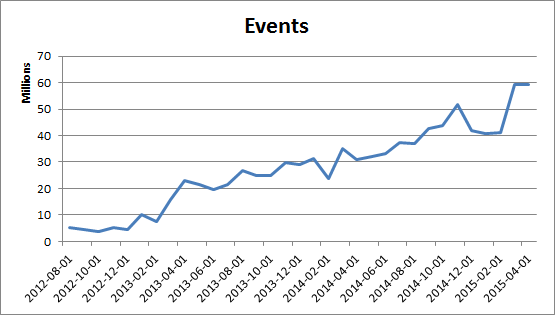
\includegraphics[]{figure/events.png}
\caption{Generated events per month. Not accumulated.}
\label{fig:events}
\end{figure}

\begin{figure}[h!]
\centering
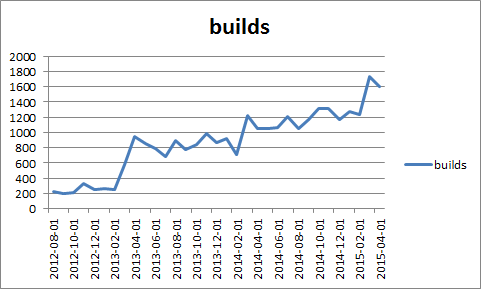
\includegraphics[]{figure/builds.png}
\caption{Generated builds per month. Not accumulated.}
\label{fig:builds}
\end{figure}

\begin{figure}[h!]
\centering
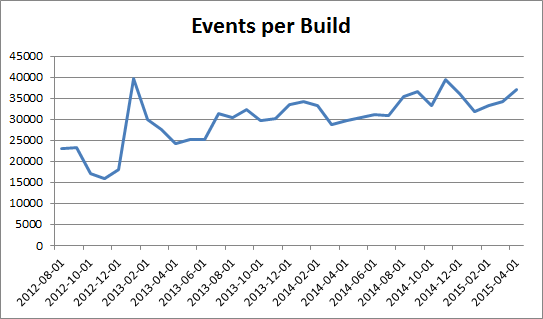
\includegraphics[]{figure/events_per_build.png}
\caption{Events per build. Not accumulated.}
\label{fig:events_per_build}
\end{figure}

%* Skriva lite här om varför det har ökat så mycket. Kanske prata med John.\\ 
%* Visa resultatet av de mätningar som gjorts om antalet build och job\_events. \\
%* Med hjälp av de mätningar så kan man skriva lite prognoser om hur mycket data som kommer genereras om 1,2 eller 5 år.

\begin{figure}[h!]
\centering
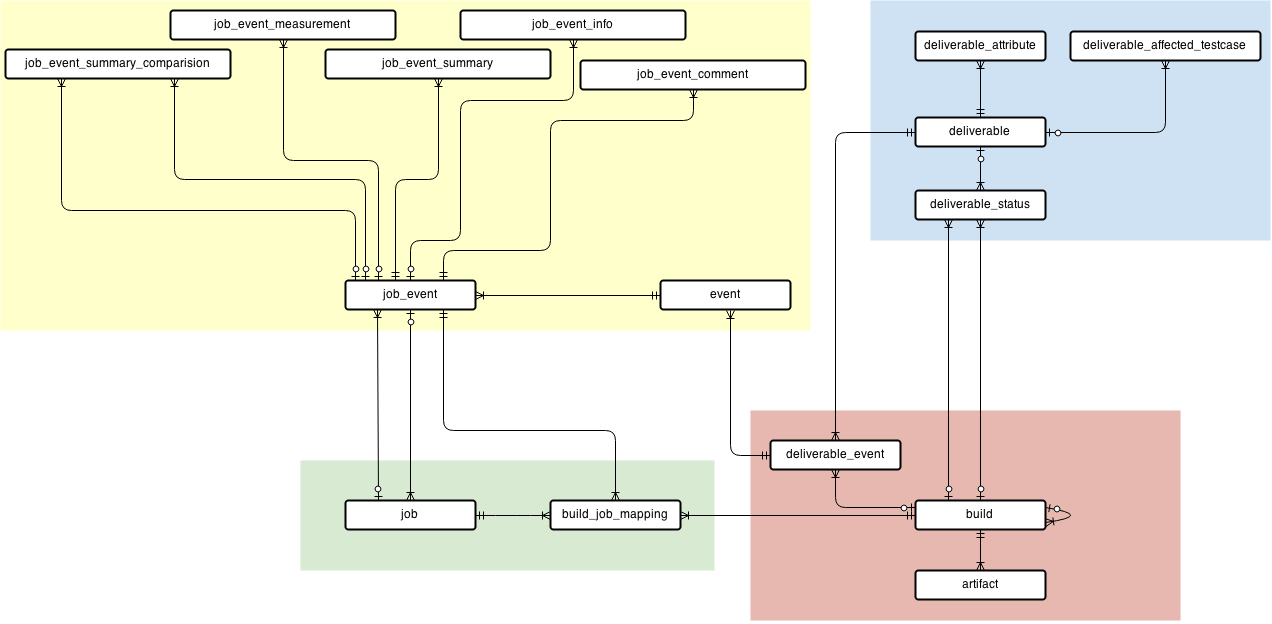
\includegraphics[scale=0.5, angle=90]{figure/sql.png}
\caption{Diagram of the relational database in CIMS.}
\label{fig:sql}
\end{figure}

%\hiddensubsubsection{Get test tree}
%\label{q:gettesttree}
%Query in CIMS: Get job tree by id or job name \\
%SQL: This query cannot be performed with a single SQL statement. The tree structure is built on the application level. Pseudo code:
%\begin{verbatim}
%job_events = SELECT * FROM cims_job_event WHERE job_name = 'some_name'
%create_tree_structure(job_events) // Recursive function
%\end{verbatim}
%Example input: $1234567$\\
%Example output: \\
%In the relational data model of CIMS, a job represents a root test suite for a specific build. I.e a test suite with no parent. This query should, given a unique id of such a job, return the hierarchical representation of that job.


%\hiddensubsubsection{Get all build data}
%\label{q:getallbuilddata}
%Query in CIMS: na \\
%SQL: This specific query is not expressed as a single SQL statement. Pseudo code:
%\begin{verbatim}
%build = SELECT * FROM cims_build WHERE id = 'some_id'
%
%jobs = 
%    SELECT cims_job.* FROM cims_job
%    INNER JOIN cims_build_job_mapping
%    ON cims_build_job_mapping.job_name = job.job_name
%    // build.id same id as previous query
%    WHERE cims_build_job_mapping.build_id = build.id
%job_names = job.name FOR job IN jobs // list comprehension
%
%job_events = SELECT * FROM cims_job_event WHERE job_name IN job_names
%\end{verbatim}
%Example input: {\tt CXS101289\_LLVDRAGON\_MKX\_SPRINT3\_R1A03\_140605084139 } \\
%Example output: \\
%This query should retrieve the complete view of a uniquely identified build. This means all the build information plus all related test suites and test cases.

%\section{Architecture of CIMS}

%CIMS has a multitier architecture as seen in figure X. Whenever a build is started, data from multiple sources is collected and sent to the system. This data is transformed to fit into the relational data model of CIMS.
%
%Presentation of data is done in real time via a web application. In order to support this, CIMS employs a number technologies in support of the main relational database, effectively forming a polyglot persistence solution. This includes a search engine (Sphinx) for aggregation of test cases, and a key value store (Redis) for caching.
%
%An external REST API is exposed to gather data for other purposes than real time visualization.